\chapter{The Hot Big Bang model}\label{chap:HotBigBang}
After having built the framework which describes the dynamics of spacetime, we shall now turn to studying the thermodynamic evolution of its constituents. \emph{Statistical mechanics} connects the dynamical evolution of each particle in the expanding universe to macroscopic observable as the temperature, the energy density or in general the energy momentum tensor. In the next sections we will develop all the machinery to describe the evolution of the \emph{phase space distribution} in curved spacetime, which leads to the \textbf{Boltzmann equation.}

As we rewind time from today, the universe shrinks and the temperature increases. Hence, the early universe was filled by a hot plasma of matter and radiation, also called \textbf{primordial plasma}. The model which describes its cooling history up to today is known as the \textbf{Hot Big Bang model}. The main result of this model, for our purpose, is that as the plasma cools down the kinetic energy of the particle decreases and thus some of them stop to interact with the other. These \emph{decoupled} particles, then evolve independently of the plasma, carrying information from their decoupling era. As we will see the \emph{CMB} is the relic of the decoupled photons. 

\section{The Boltzmann equation}\label{sec:BoltzmannEquation}
The expansion of the universe influences dynamically the motion of all the particles it contains, for example redshifting photon's frequency, hence also the corresponding energy and the momentum. This is also reflected in the thermodynamic observables (for instance as the photon energy gets redshifted their temperature must decrease). 

As far as we don't consider quantum mechanics, the state of a many-particle system is totally described by their positions and local momenta\footnote{The following treatment could also be done using the comoving momenta, in the end the resulting equations would have been a little different.} $(\mathbf x_i,\mathbf p_i)$, which for $N$ particles corresponds to $6N$ numbers. Already considering systems on the Earth this number becomes quite large, making unsolvable the exact dynamics of all these particles. Statistical mechanics builds then on the idea that all the macroscopic observables can be obtained from the statistics of the microscopic ones. This can be achieved by introducing a \textbf{phase space distribution} $f(\mathbf x,\mathbf p, t)$ and then averaging over the phase space. In general, we define
\begin{equation}
    \label{eq:phspace_dist}
    dN(\mathbf x,\mathbf p, t)=f(\mathbf x,\mathbf p, t) \frac{d^3x\ d^3p}{(2\pi)^2},
\end{equation}
where $dN(\mathbf x,\mathbf p, t)$ is the number of particles in the state $(\mathbf x,\mathbf p)$ at the instant $t$ and the factor $d^3x\ d^3p/(2\pi)^2$ is the phase space measure normalized by the \emph{Planck's constant}, which in natural units reads $h=(2\pi)^{3}$. The thermodynamic evolution of the system is then determined by how $f(\mathbf x,\mathbf p, t)$ changes over time: this is described by the \textbf{Boltzmann equation}
\begin{equation}
    \label{eq:Boltzmann}
    \hat{L}[f]=C[f],
\end{equation}
where we introduced the two operators $\hat{L}$ and $C$. The former is called \textbf{Liouville operator} and it is defined as the total derivative with respect to time of $f$, while the latter is the \textbf{collision operator} which instead describes and depends on the interactions of the system. The effects of gravity are not considered interactions in general relativity (since gravity is not a force) and instead influences the system through the Liouville operator: indeed, by the chain rule we have 
$$ 
\hat{L}[f]\defeq\frac{df}{dt}(\mathbf x,\mathbf p, t)= \frac{\partial f}{\partial t}+\frac{\partial f}{\partial x^i}\frac{dx^i}{dt}+\frac{\partial f}{\partial p^i}\frac{dp^i}{dt},
$$ 
the explicit form of this equation will show explicitly the dependence on the evolution of spacetime. For now, we are just considering an isotropic and homogeneous universe, hence we cannot expect $f$ to depend on a specific position $\mathbf{x}$ nor on a specific direction $\versor p$ (namely particles momenta can have different directions of motion but macroscopically no preferred direction should be distinguishable) and thus the equation above reduces to 
$$
\hat{L}[f]\defeq\frac{df}{dt}(p, t)= \frac{\partial f}{\partial t}+\frac{\partial f}{\partial p}\frac{dp}{dt}.
$$ 
The only term we should compute is $\tfrac{dp}{dt}$: this can be obtained by the geodesic equation in FRW universe. Recalling that $p$ is the modulus of the local 3-momentum, which is defined such that the mass-shell condition of flat spacetime holds
\begin{align*}
    m^2=-P^\mu P_\mu=(P^0)^2-a^2(t)P^iP^j\delta_{ij}=E^2-p^ip^j\delta_{ij}\quad\Rightarrow\quad
    \begin{cases}
        E\defeq P^0\\
        p^i\defeq a P^i
    \end{cases},
\end{align*}
where a different metric would lead to a different definition of local energy ($E$) and momentum, the geodesic equation gives
\begin{align*}
    &\frac{dP^i}{dt}=-\Gamma^{i}_{\mu\nu}\frac{P^\mu P^\nu}{P^0}=-2\Gamma^{i}_{j0}P^j=-2HP^i\\
    &\Rightarrow\quad \frac{dp}{dt}=H p+a\frac{d}{dt}\sqrt{P^iP^j\delta_{ij}}=Hp+\frac{ap^i}{p}\frac{dP^j}{dt}\delta_{ij}=-Hp,
\end{align*}
where we used that the only non-vanishing Christoffel symbol with an upper spatial index must have just one lower spatial index. Putting all together we find the Liouville operator for a homogeneous and isotropic universe
\begin{equation}
    \label{eq:Homo_Iso_Liouville}
    \hat L[f]=\frac{\partial f}{\partial t}-Hp\frac{\partial f}{\partial p}.
\end{equation}
Since the explicit form of the collision operator depends on the physics of the different components of the universe, we won't focus here on the derivation of such term. 
\subsection{Thermodynamic observables}
\label{sec:thdm_obs}
Having sketched the way in which the phase space distribution can be obtained, we now have to describe how to compute the macroscopic observables that describe the plasma that filled the universe. 

We already know, form the definition \eqref{eq:phspace_dist}, that integrating over phase space $f$ yields the total number of particles. When dealing with the whole universe, computing extensive quantities is not very convenient, instead integrating only over momentum space clearly yields intensive quantities (e.g. number density $n\defeq N/V$). The immediate generalization of \eqref{eq:phspace_dist} is the \emph{particle current density}
\begin{equation}
    N^\mu\defeq\frac{g_\text{dof}}{(2\pi)^3\sqrt{-g}}\int d^3P\frac{P^\mu}{P^0} f(p,t)=\frac{g_\text{dof}}{(2\pi)^3}\int d^3p\frac{P^\mu}{P^0} f(p,t),
    \label{eq:current_density}
\end{equation}
where we introduced the degeneracy factor $g_\text{dof}$ which counts the number of internal degrees of freedom of the particles (e.g. $g_\text{photons}=2$).  We recognize that the zeroth component corresponds to the number density $n$ while the spatial components represent the 3-current density $\mathbf j$\footnote{Note that $\mathbf j=0$ to have isotropy.}. Indeed, imposing the conservation of the particle current density we recover the conservation of the particle number
\begin{align*}
    0=\tensor{N}{^\mu_;_\mu}&=\frac{g_\text{dof}}{(2\pi)^3a^3}\frac{\partial }{\partial t}\bigg(a^3\int d^3p\frac{P^0}{P^0}f\bigg)=\frac{g_\text{dof}}{(2\pi)^3}\bigg[3H\int d^3p\ f+ \int d^3p\frac{\partial f}{\partial t}\bigg]\\&=\frac{g_\text{dof}}{(2\pi)^3}\bigg[3H\int d^3p\ f+H\int d^3p\ p\frac{\partial f}{\partial p}+ \int d^3p\ \hat L[f]\bigg]\\
    &\bigg\downarrow\ \text{Integrating by parts the second term}\\
    &=\frac{g_\text{dof}}{(2\pi)^3}\int d^3p\ \hat L[f]\\
    &\Rightarrow\qquad \boxed{\frac{1}{a^3}\frac{\partial (a^3n)}{\partial t}=\frac{g_\text{dof}}{(2\pi)^3}\int d^3p\ \hat L[f]=\frac{g_\text{dof}}{(2\pi)^3}\int d^3p\ C[f]},
\end{align*} 
where in the first line we used that the 4-divergence of a 4-vector is $\tensor{A}{^\mu_;_\mu}=\tfrac{1}{\sqrt{-g}}\tfrac{\partial (\sqrt{-g}A^\mu)}{\partial x^\mu}$. In absence of interactions, that could source or remove particles, this reduces to the requirement that the number of particle in a given volume is fixed, namely $a^3 n=$ const.

Similarly, the energy-momentum tensor can be redefined as a function of the phase space distribution
\begin{equation}
    \tensor{T}{^\mu_\nu}\defeq \frac{g_\text{dof}}{(2\pi)^3\sqrt{-g}}\int d^3P\frac{P^\mu P_\nu}{P^0}f(p,t)=\frac{g_\text{dof}}{(2\pi)^3}\int d^3p\frac{p^\mu p_\nu}{p^0}f(p,t),
    \label{eq:SressEnergyT_phasespace}
\end{equation}
where $p^0\defeq E$. The above expression allows computing the energy density and the pressure of the corresponding cosmic fluid.

Overall we shall recall two quantities
$$
n=\frac{g_\text{dof}}{(2\pi)^3}\int d^3p\ f(p,t),\qquad \rho=\frac{g_\text{dof}}{(2\pi)^3}\int d^3p\ E\ f(p,t),
$$
which we will use extensively in the next sections.
\subsection{Equilibrium distributions} \label{sec:EquilibriumDistributions}
Determining macroscopic observable can become rather non-trivial when considering systems which are not in equilibrium. We will see that the early universe, due to the high efficiency of the interactions in the plasma, can be approximately considered as a system in equilibrium. This simplification allows obtaining analytic results that can already grasp the main features of the evolution of the plasma. Further improvements can be achieved numerically or by means of perturbation theory, however we will not focus on these here.\\
In general, the equilibrium distribution is a stationary solution $\tfrac{\partial f}{\partial t}=0$, not to be confused with the condition $\tfrac{d f}{dt}=0$. If we consider the \emph{collisionless case} ($C[f]=0$) the equilibrium distribution is determined completely by the initial condition of the system (since now the Boltzmann equation gives us $f=$ const). However, in presence of interactions the distribution will be determined by the collision operator too. 

Let's consider the interaction rate $\Gamma$ associated to the interactions in the plasma, for large values of $\Gamma$ we expect to have also a large contribution from $C[f]$ in the Boltzmann equation. The effects of gravity in the Boltzmann equations are instead proportional to the Hubble parameter $H$ (see equation \eqref{eq:Homo_Iso_Liouville}). In this way we can understand that, as a first approximation, in the limit $\Gamma\gg H$ the effects of the expansion of the universe become negligible and we can use well-known phase space distributions, while when $\Gamma\ll H$ the interactions are negligible and only the expansion will influence the system for which holds the conservation of particles we previously obtained. When a particular component of the universe transitions from the first case to the second, we usually say that it \emph{freezes-out}. In general, we can expect the interaction rate to be proportional to the number density of particle while we know that the Hubble parameter is instead a decreasing function of time ($H\propto t^{2/(3+3\omega)-1}$), this means that initially, when the universe was denser, the phase space was mainly influenced by interactions, while at later times different species started to freeze-out and to cool down as the universe expanded.

When the interactions are dominant and equilibrium is met, we expect to obtain a \textbf{Bose-Einstein} distribution or a \textbf{Fermi-Dirac} distribution, respectively for bosons and fermions
\begin{equation}
    \label{eq:BE_FD_distributions}
    f(p)=\bigg[\exp\bigg\{\frac{E(p)+\mu}{k_BT}\bigg\}\pm1\bigg],\qquad (+) \text{ for fermions and } (-)\ \text{for bosons.}
\end{equation}
In the above it appears the \emph{chemical potential} $\mu$, which measures the energy needed to remove or insert a new particle in the system and it can be temperature dependent. Knowing the phase space distribution we can now compute the number density and the energy density, however their exact expression can be hard to be found. We will therefore focus on two physically meaningful limits: the \textbf{ultrarelativistic limit} $T\gg m$, in which the particles behave as radiation, and the \textbf{non-relativistic limit } $T\ll m$, for which we recover the classical behavior.
\subsubsection{Ultrarelativistic limit}
Very light particles, such as neutrinos, or with a large momentum (compared to their rest mass) can be approximated to be massless as photons. Hence, the mass-shell condition implies that $E=p$, moreover we will assume that the chemical potential is negligible for these species. This last assumption is reasonable considering that at equilibrium, in presence of interactions that can change the number of particles, $\mu$ should vanish. Under these assumptions we can compute the number density of ultrarelativistic particles 
\begin{align*}
    n&=\frac{g_\text{dof}}{(2\pi)^3}\int d^3p\ \frac{1}{\exp(\frac{p}{k_BT})\pm1}=\frac{g_\text{dof}}{2\pi^2}\int_0^\infty dp \frac{p^2 }{\exp(\frac{p}{k_BT})\pm1}=\frac{g_\text{dof}}{2\pi^2}(k_BT)^3\int_0^\infty dx \frac{x^2}{e^x\pm1},
\end{align*}
    here we can observe that the fermionic (+) case can be obtained from the calculations for bosons (-) by
    $$
        \frac{1}{e^x+1}=\frac{1}{e^x-1}-\frac{2}{e^{2x}-1},
    $$
    performing the change of variable $2x\rightarrow x$ in the second term we find that the fermionic integral is $1-2(1/2)^3=3/4$ the bosonic one. Exploiting the geometric series, the bosonic integral yields
\begin{align*}
   \frac{g_\text{dof}}{2\pi^2}(k_BT)^3\int_{0}^{\infty}dx\frac{x^2e^{-x}}{1-e^{-x}}  &=\frac{g_\text{dof}}{2\pi^2}(k_BT)^3\int_0^\infty dx\ x^2e^{-x}\sum_{n=0}^{\infty} e^{-nx}\nonumber\\&=\frac{g_\text{dof}}{2\pi^2}(k_BT)^3\sum_{n=0}^{\infty}\frac{2}{(n+1)^3}\xrightarrow[\text{Riemman zeta function}]{\zeta(z)\defeq\sum_{n=1}^\infty n^{-z}}\frac{g_\text{dof}}{\pi^2}\zeta(3)(k_BT)^3.
\end{align*}
From our previous observation we conclude that
\begin{equation}
    n=\frac{g_\text{dof}}{\pi^2}\zeta(3)(k_BT)^3\begin{cases}
        1\quad \text{bosons},\\
        \frac{3}{4}\quad \text{fermions.}
    \end{cases}
    \label{eq:relativistic_number_density}
\end{equation}
Similarly, the energy density reads
\begin{align*}
    \rho&=\frac{g_\text{dof}}{(2\pi)^3}\int d^3p\ \frac{E}{\exp(\frac{p}{k_BT})\pm1}=\frac{g_\text{dof}}{2\pi^2}\int_0^\infty dp \frac{p^3 }{\exp(\frac{p}{k_BT})\pm1}=\frac{g_\text{dof}}{2\pi^2}(k_BT)^4\int_0^\infty dx \frac{x^3}{e^x\pm1},
\end{align*}
         where this time the fermion integral (+) turns out to be $1-2(1/2)^4=7/8$ the bosonic one. Proceeding with the calculations for bosons we find
\begin{align*}
   \frac{g_\text{dof}}{2\pi^2}(k_BT)^4\int_{0}^{\infty}dx\frac{x^3e^{-x}}{1-e^{-x}}  &=\frac{g_\text{dof}}{2\pi^2}(k_BT)^4\int_0^\infty dx\ x^3e^{-x}\sum_{n=0}^{\infty} e^{-nx}\nonumber\\&=\frac{g_\text{dof}}{2\pi^2}(k_BT)^4\sum_{n=0}^{\infty}\frac{6}{(n+1)^4}\xrightarrow[\text{Riemman zeta function}]{\zeta(z)\defeq\sum_{n=1}^\infty n^{-z}}3\frac{g_\text{dof}}{\pi^2}\zeta(4)(k_BT)^4.
\end{align*}
Using that $\zeta(4)=\pi^4/90$ we have
\begin{equation}
    \rho=\frac{\pi^2}{30}g_\text{dof}(k_BT)^4\begin{cases}
        1\quad \text{bosons},\\
        \frac{7}{8}\quad \text{fermions.}
    \end{cases}
    \label{eq:relativistic_energy_density}
\end{equation}
In appendix \ref{sec:SmallChemicalPotential} expressions for the energy and number densities are computed in presence of a small chemical potential for bosons. 
\subsubsection{Non-relativistic limit}
Heavy particles at low temperature, namely $T\ll m$, (which corresponds to low momenta) behave classically, as we can see expanding the relativistic kinetic energy
$$
E(p)=\sqrt{p^2+m^2}\approx m+ \frac{1}{2m}p^2+\mathcal{O}(p^2).
$$ 
In this limit both Bose-Einstein and Fermi-Dirac distributions reduce to the \textbf{Boltzmann} distribution
$$
f(p)=\bigg[\exp\bigg\{\frac{E(p)+\mu}{k_BT}\bigg\}\pm1\bigg]\xrightarrow{T\ll m}e^{-\frac{E(p)+\mu}{k_BT}}\approx e^{-\frac{m+\mu}{k_BT}}e^{-\frac{p^2}{2mk_BT}}.
$$
Under this approximation, both the integral for the number denisty and of the energy density become Gaussian integrals
\begin{align}
    n&=\frac{g_\text{dof}}{(2\pi)^3}\int d^3p\ \frac{1}{\exp(\frac{E(p)+\mu}{k_BT})\pm1}\approx\frac{g_\text{dof}}{2\pi^2}e^{-\frac{m+\mu}{k_BT}}\int_{0}^{\infty}dp\ p^2  e^{-\frac{p^2}{2mk_BT}}\nonumber\\
    &=\frac{g_\text{dof}}{2\pi^2}e^{-\frac{m+\mu}{k_BT}}(mk_BT)^{\frac{3}{2}}\int_{0}^{\infty}dx\ x^2  e^{-\frac{x^2}{2}}=g_\text{dof}\bigg(\frac{mk_BT}{2\pi}\bigg)^{\frac{3}{2}}e^{-\frac{m+\mu}{k_BT}},\label{eq:nonrel_number_density}\\
    \rho&=\frac{g_\text{dof}}{(2\pi)^3}\int d^3p\ \frac{E}{\exp(\frac{E(p)+\mu}{k_BT})\pm1}\approx\frac{g_\text{dof}}{2\pi^2}e^{-\frac{m+\mu}{k_BT}}\int_{0}^{\infty}dp\ p^2  e^{-\frac{p^2}{2mk_BT}}\bigg(m+\frac{p^2}{2m}\bigg)\nonumber\\
    &=nm+\frac{nT}{2}\bigg[\sqrt{\frac{2}{\pi}}\int_{0}^{\infty}dx\ x^4  e^{-\frac{x^2}{2}}\bigg]=nm+\frac{3}{2}nT.
\end{align}
Notice that in the non-relativistic case the number and energy densities are exponentially suppressed at high temperatures while in the relativistic limit we have that both are monotonically increasing with the temperature
\section{Primordial plasma}
As we already mentioned, at the earliest times our universe was filled by a hot plasma of interacting particles. We now know that these species can be described as relativistic particles: initially all the interactions are quite efficient and the plasma is kept at equilibrium. Then, as the universe cools down, some species start to become non-relativistic and their contributions to the energy and number to be exponentially suppressed. Moreover, at high temperature ($T\gg m$) particle-antiparticle pairs production is sustainable counterbalancing their annihilation. Instead, once the temperature drops below the mass of a specific species pair production stops and they annihilate.

In general, the total energy density of the universe depends on the temperature and on the degeneracy factor of each species
\begin{equation}
    \rho=T^4\bigg[\sum_{\text{Bosons}}g_i\bigg(\frac{T_i}{T}\bigg)^4+\frac{7}{8}\sum_{\text{Fermions}}g_j\bigg(\frac{T_j}{T}\bigg)^4\bigg]\defeq g_{*}(T)T^4, \label{eq:total_energy_density}
\end{equation}
where the indexes $i$ and $j$ run over the bosonic and fermionic species respectively. In the above we defined the \emph{effective number of relativistic degrees of freedom} $g_*$, note that this quantity depends on the temperature of all the species in the plasma. When all the different species are in equilibrium $g_*$ counts the total number of relativistic degrees of freedom. Considering the \emph{Standard Model of particles} the total number of degrees of freedom are divided in the following way.
\begin{itemize}
    \item \textbf{Gauge bosons}, which are the carrier of the three fundamental interactions, are all spin-1 particles: photons and the eight gluons of the QCD are massless thus they have 2 d.o.f. each, while the $W^\pm$ and $Z$ bosons of the Weak interaction being massive posses 3 d.o.f. each. On top of these, we must add the \textbf{Higgs boson}, which is a scalar spin-0 field, thus having one single internal degree of freedom. Overall the total number of bosonic d.o.f is
    $$g_\text{Bosons}=2\times 9+3\times3+1= 28.$$
    \item \textbf{Fermions} are instead the particles responsible for the matter we observe in the universe and they are all massive spin-$1/2$ particles. \textbf{Charged leptons} ($e^\pm,\mu^\pm,\tau^\pm$) are massive charged particles, each flavor (e.g. electron, muon, \dots) has 2 d.o.f. for each spin state. The electric charge allows for antiparticles to exist, doubling the d.o.f. to $3\times2\times2=12$. \textbf{Quarks} ($t,b,c,s,d,u$), on top of the electric charge, posses also a \emph{color charge} (blue, red, green) resulting in $6\times2\times2\times3=72$ degrees of freedom. Lastly, \textbf{neutrinos} ($\nu_e,\nu_\mu,\nu_\tau$) do not possess any charge, however understanding the number of internal d.o.f. they possess is more involved. Indeed the Standard Model predicts three massless neutrinos, to respect its gauge symmetries, however we now know that they have a small mass, even though we still don't know whether they have a \emph{Majorana mass} or a \emph{Dirac mass}. Observations suggest that only 2 d.o.f for each flavor influence the primordial plasma, this could be explained or by having a Majorana mass (which would make the neutrino being its own antiparticle) or by assuming that, having a Dirac mass, the antineutrinos decoupled from the plasma at very early times. Overall the degrees of freedom of fermions are
    $$
    g_\text{fermions}=3\times2\times2+6\times2\times2\times3+6=90.
    $$
\end{itemize}
Summing all together and accounting for the difference between bosons and fermions we find
\begin{equation}
    g_*=g_\text{Bosons} + \frac{7}{8}\ g_\text{Fermions}=106.75
    \label{eq:relativ_dof}
\end{equation}
\subsection{Annihilation and decoupling of species}
\label{sec:decoupling}
As we already explained, as the primordial plasma cools down and the temperature drops below the mass of a species, the pair-production process stops and the species annihilates reducing the number of relativistic degrees of freedom of the plasma.  
The heaviest particle of the Standard Model is the \emph{top quark}, with $m_t=171$ GeV, and thus it annihilates first. Then the \emph{Higgs} ($125$ Gev) and the \emph{gauge bosons} annihilate, followed by the \emph{bottom quark}. After the \emph{charm quark} and the \emph{tauon} annihilated, right before the turn of the \emph{strange quark}, \textbf{QCD phase transition} occurs: at $T\sim 150$ Mev the remaining quarks combine into baryons (protons, neutrons, \dots) and mesons (pions, \dots). All the resulting species, except the pions ($\pi^\pm,\pi^0$) are non-relativistic at this temperature and thus exponentially suppressed, leaving in large number in the plasma only pions, electrons, muons, neutrinos and photons. The three types of pions are spin-0 bosons with 1 d.o.f each: after QCD phase transition the relativistic degrees of freedom are just $g_*=2+3+\tfrac{7}{8}\times(4+4+6)=17.254$. As the universe continues cooling down \emph{muons} and \emph{pions} annihilate leading to $g_*=10.75$. At this point in the thermal history of our universe some interactions start to stop (the expansion rate $H$ dominates over $\Gamma$) and the next species will \textbf{decouple} without annihilation.

\begin{figure}
\centering
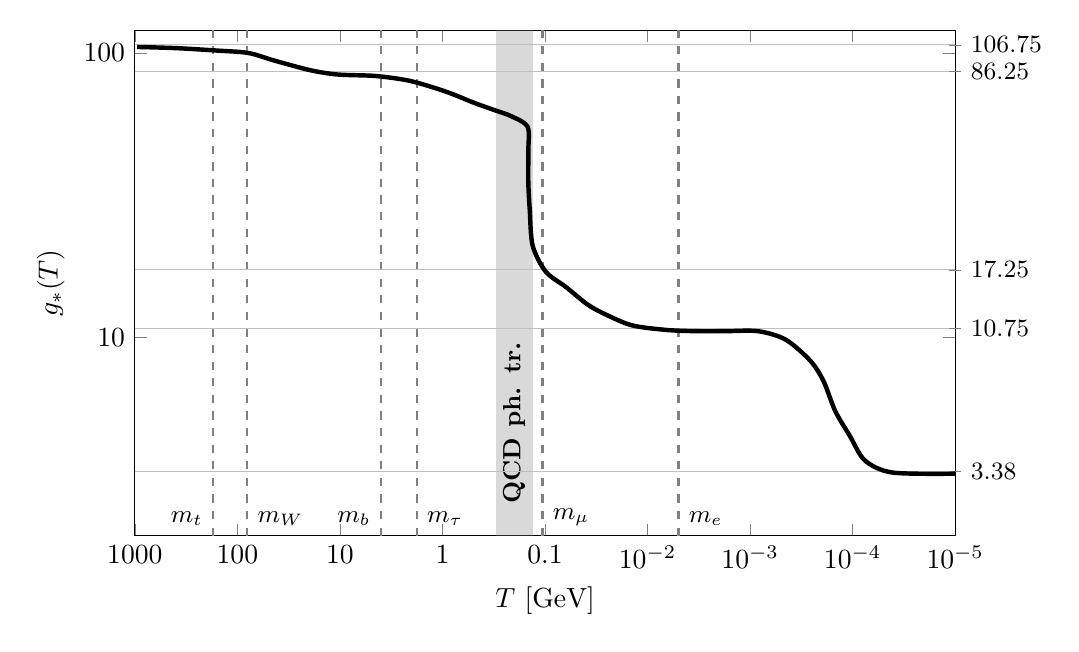
\begin{tikzpicture}
  \begin{axis}[
    width=12cm, height=8cm,
    xlabel={\(T\) [GeV]},
    ylabel={\(g_*(T)\)},
    xmin=1e-5, xmax=1e3,
    ymin=2, ymax=120,,
    x dir=reverse,
    xmode= log,
    ymode=log,
    xtick={1000.0,100.0,10.0,1,.1,0.01,0.001,0.0001,0.00001},
    xticklabels={1000,100,10,1,0.1,$10^{-2}$,$10^{-3}$,$10^{-4}$,$10^{-5}$},
    ytick={100.0, 10.0},
    yticklabels={100,10},
  ]
        % Vertical lines for particle masses
    \draw[dashed, gray, thick] (axis cs:173,2)node[black, above left, font=\small,  anchor=south east] {$m_t$} -- (axis cs:173,120) ;
    \draw[dashed, gray, thick] (axis cs:80,2)node[black, above right, font=\small,  anchor=south west] {$m_W$} -- (axis cs:80,120) ;
    \draw[dashed, gray, thick] (axis cs:4,2)node[black, above, font=\small,  anchor=south east] {$m_b$} -- (axis cs:4,120) ;
    \draw[dashed, gray, thick] (axis cs:1.777,2)node[black, above, font=\small,  anchor=south west] {$m_\tau$} -- (axis cs:1.777,120) ;
    \draw[dashed, gray, thick] (axis cs:0.106,2)node[black, above, font=\small,  anchor=south west] {$m_\mu$} -- (axis cs:0.106,120) ;
    \draw[dashed, gray, thick] (axis cs:0.005,2)node[black, above, font=\small,  anchor=south west] {$m_e$} -- (axis cs:0.005,120) ;

    \addplot [
        domain=0.13:0.3,
        samples=2,
        fill=gray,
        opacity=0.3,
        draw=none
    ] {120} \closedcycle;
    
    \path (axis cs:0.2,5) node[rotate=90, color=black, font=\bfseries\small] {QCD ph. tr.};
  \end{axis}

    \begin{axis}[
    width=12cm, height=8cm,
    xmin=1e-5, xmax=1e3,
    ymin=2, ymax=120,
    x dir=reverse,
    xmode=log,
    ymode=log,
    axis line style={draw=none},
    axis y line=right,
    axis x line=none,
    ytick={106.75,86.25,17.25,10.75,3.38},
    yticklabels={106.75,86.25,17.25,10.75,3.38},
    ymajorgrids=true,
    tick label style={anchor=west, font=\small},
    grid=major,
    % Hide everything else except y-ticks and grid
    xtick=\empty,
    xlabel={},
    ylabel={},
    title={},
    legend style={draw=none},
    % Do NOT use hide axis!
  ]
  \addplot[ultra thick, smooth] table {
      % T (GeV)    g*
    952.1895354084076 105
    394.22547112067946 104
    160.57345752835954 102
    78.27390868337491 100
    43.480834671045116 94
    19.533503372283345 87
    10.502110796366669 84
    4.492439834714388 83
    2.1544346900318843 80
    1.139561028855787 75
    0.7453159674382293 71
    0.5036486330526275 67
    0.31365621741294075 63
    0.21544346900318845 60
    0.147983319823753 55
    0.14558631963371274 45
    0.14558631963371274 35
    0.14090816855117316 28
    0.1319980075832034 21
    0.09838022272179395 17
    0.06227679315078501 15
    0.03815577539950052 13
    0.025366194557577992 12
    0.014090816855117316 11
    0.006434438263328995 10.6
    0.003294052347239973 10.5
    0.001742347400593542 10.5
    0.0008355757272293571 10.5
    0.00044924398347143926 9.8
    0.0002578383526261189 8.25
    0.00019217104123021506 7
    0.000147983319823753 5.5
    0.00010675022383376014 4.5
    0.00007575871926473297 3.68
    0.00004073137564447355 3.34
    0.00001 3.31
    };
  \end{axis}
\end{tikzpicture}
\caption{Evolution of the effective number of relativistic degrees of freedom $g_{*}$ as a function of the temperature in the early universe.}
\label{fig:gstar}
\end{figure}

The first interactions to stop, at around $T\sim 1$ MeV, is the Weak interaction of neutrinos such as
$$ \nu_e+\bar\nu_e\rightleftharpoons e^++e^-.$$
After decoupling the collision term of neutrinos is negligible and thus the number of neutrinos is conserved: this shows that neutrinos then start to cool as 
$$\text{const}=na^3\propto T_\nu^3a^3\qquad\Rightarrow \qquad T_\nu\propto a^{-1},$$
independently to what happens at the rest of the plasma. The relic of these neutrinos is also called \emph{cosmic neutrino background} (C$\nu$B).

Shortly after neutrino decoupling, the temperature reaches the electron mass and thus electron/positron annihilation occurs producing photons
$$e^++e^-\quad\longrightarrow\quad \gamma+\gamma.$$ In this process the energy of the annihilated electrons is transferred to photons heating them a bit resulting in a slightly colder relic of neutrinos compared to photons. At this point some electron survived the annihilation due to an initial \emph{matter-antimatter asymmetry}, which origin is still unclear.

As the universe continues to cool down the temperature reaches the bound energy of Hydrogen atoms thus allowing for the remaining free electrons and nuclei (formed by interaction of protons and neutrons) to bound. 
\subsection{Recombination}\label{sec:recombination}
The phase in which the first atoms formed is called \textbf{recombination}: at this point in time only electrons that survived the annihilation and nuclei were part of the plasma. Around $90\%$ of the nuclei in the plasma are just protons and thus they will form with electrons Hydrogen atoms. The remaining nuclei will instead form Helium atoms, which we are going to neglect here. 

To study the reaction that results into Hydrogen,
$$
e^-+p^+ \rightleftharpoons H+ \gamma,
$$
we will consider a universe filled only by $e^-,\ p^+$ and $H$ all in the non-relativistic regime $T\ll m_i$. At equilibrium the number density of these three species is given by equation \eqref{eq:nonrel_number_density}: in the end we want to find the temperature at which recombination occurs, namely when $n_H\gg n_e,n_p$. A way to compare these three densities is by constructing the following ratio
$$
\frac{n_H}{n_en_p}\bigg|_\text{eq}=\frac{g_H}{g_eg_p}\bigg(\frac{m_H}{m_em_p}\frac{2\pi}{k_BT}\bigg)^{\frac{3}{2}}\exp\bigg(\frac{m_p+m_e-m_H}{k_bT}\bigg),
$$
where we used the \eqref{eq:nonrel_number_density} and we imposed that $\mu_e+\mu_p=\mu_H$ to have equilibrium. Notice that this construction gives us automatically the quantity
$$
E_I\defeq m_p+m_e-m_H=13.6\text{ eV}
$$
which turns out to be the \emph{ionization energy of the Hydrogen atom}, namely the energy needed to remove the electron from the ground state of H. The internal degrees of freedom of both protons and electrons are 2 (the 2 $\tfrac12$-spin states) while for H they are 4, as they correspond to the states allowed by the sum of the spins of $e$ and $p$, which are a singlet of spin 0 and a triplet of spin 1.  Exploiting that $m_H\approx m_p$ and that the universe isn't electrically charged ($n_e=n_p$) the above reads
$$
\frac{n_H}{n_e^2}\bigg|_\text{eq}=\bigg(\frac{2\pi}{m_ek_BT}\bigg)^{\frac{3}{2}}\exp\bigg(\frac{E_I}{k_bT}\bigg).
$$
Instead of studying this equation in the limit in which the free electrons are zero, it is often defined the \textbf{free-electron fraction}, which represents the fraction of free electrons over the Hydrogen atoms (both neutral and ionized),
\begin{equation}
    X_e\defeq\frac{n_e}{n_p+n_H}=\frac{n_e}{n_e+n_H}\quad\Rightarrow\quad \frac{1-X_e}{X_e^2}=\frac{n_H}{n^2_e}(n_e+n_H)\defeq\frac{n_H}{n^2_e}n_b,
\end{equation}
where we used the number density of baryons $n_b$. The main advantage is that the \textbf{baryon-to-photon ratio} $\eta_{b\gamma}\defeq n_b/n_\gamma$ from now on is conserved and we can easily compute $n_\gamma$ from equation \eqref{eq:relativistic_number_density} finding
\begin{equation}
    \frac{1-X_e}{X_e^2}\bigg|_\text{eq}=\frac{2\zeta(3)}{\pi^2}\eta_{b\gamma}\bigg(\frac{2\pi k_BT}{m_e}\bigg)^{\frac{3}{2}}\exp\bigg({\frac{E_I}{k_BT}}\Bigg),\label{eq:Saha}
\end{equation}
which is the \textbf{Saha equation}. We can solve the above for $X_e$ to find
$$
X_e\bigg|_\text{eq}=\frac{-1+\sqrt{1+4f}}{2f}\qquad \text{with }f(T,\eta)=\frac{2\zeta(3)}{\pi^2}\eta\bigg(\frac{2\pi k_BT}{m_e}\bigg)^{\frac{3}{2}}\exp\bigg({\frac{E_I}{k_BT}}\Bigg),
$$
which is shown in Figure \ref{fig:saha}.
\begin{figure}[ht!]
\centering
\begin{tikzpicture}
  \begin{axis}[
    width=10cm, height=7cm,
    xlabel={$T$ [eV]},
    ylabel={$X_e$},
    xmin=0.25, xmax=0.4,
    ymin=0, ymax=1,
    domain=0.1:1.5,
    samples=200,
    xtick={0.25,0.3,0.35,0.4, 0.32},
    xticklabels={0.25,0.3,0.35,0.4, $T_\text{rec}$},
    ytick={1,0.75,0.5,0.25},
    % Make axis arrows bigger
    axis line style={->, >=stealth},
  ]
    % Saha function
    \addplot [
      color=black, thick,
      domain=0.01:0.5,
      samples=200,
    ]
    { 
     (-1+sqrt(1+8*1.2/9*6E-10*(6*x/5.11E5)^1.5*e^(13.6/x)))/(4*1.2/9*6E-10*(6*x/5.11E5)^1.5*e^(13.6/x))
    };
  \end{axis}
  \begin{axis}[
    width=10cm, height=7cm,
    xmin=0.25, xmax=0.4,
    ymin=0, ymax=1,
    axis x line=top,
    axis y line=none,
    xtick={0.28, 0.325, 0.37, 4.18},
    xticklabels={1200, 1400, 1600, 1800},
    tick label style={font=\small},
    ytick=\empty,
    xlabel={$z$},
    ylabel={},
    title={},
    legend style={draw=none},
  ]
  \draw[dashed, gray, thick] (axis cs:0.32,0) -- (axis cs:0.32,1) ;
  \end{axis}
\end{tikzpicture}
\caption{Free electron fraction $X_e$ as a function of temperature $T$ (in eV) and redshift for $\eta=6\times10^{-10}$ and $E_I=13.6$ eV. From the graph we can appreciate when recombination occurs.}
\label{fig:saha}
\end{figure}
We can appreciate that the fraction of free electrons drops at around $T\approx 0.32$ eV $\approx3760$ K, that is one order of magnitude lower than the ionization energy of Hydrogen. Recombination is delayed to when the plasma reaches this lower temperature because the number of free photons is far greater than the number of Hydrogen atoms, which means that even at $T<E_I$ a non-negligible fraction of photons have still $E_\gamma>E_I$, being in the tail of their energy distribution.
Knowing that the temperature of photons today (CMB) is $T_\gamma\approx2.73$ K and that $T_\gamma\propto a^{-1}$ (since as we will see right after recombination photon decoupling occurs), we can compute the redshift at which Hydrogen formed
$$
1+z_\text{rec}=\frac{T_\text{rec}}{T_{\gamma,0}}\approx 1380.
$$
Similarly, we can compute the duration of recombination, which is $\Delta z\approx 80$, or $\Delta t\approx 7\times 10^{4}$ years, to go from $X_e=0.9$ to $0.1$. Note that recombination occurs entirely during the matter-dominated era, as $z_\text{rec}<z_\text{eq}=3400$.

We conclude by mentioning that the estimate we found can be further refined considering the non-equilibrium solution of the Boltzmann equation, since as the fraction of free electrons decreases it gets harder to maintain equilibrium. The full calculation would show that recombination gets delayed to $z_\text{rec}\approx 1270$.
\subsection{Photon decoupling and the CMB}
\label{sec:CMB_decoupling}
Until recombination photons were kept in equilibrium with the rest of the plasma mainly through \emph{Compton scattering}
$$
e^-+\gamma\rightleftharpoons e^-+\gamma 
$$
which we will discuss in more detail in chapter \ref{chap:SpectralDistortions}. As we will see, the interaction rate for this process can be estimated as $\Gamma_\gamma\approx n_e\sigma_T$, where $\sigma_T\approx2\times 10^{-3}$ MeV$^{-2}$ is the Thompson cross-section, therefore decoupling depends on the number of free electrons in the universe. In the previous section we studied the evolution of this quantity discovering that at recombination the fraction of free electrons drops to zero, in this way the interaction rate will eventually become smaller than the expansion rate of the universe. We know that at that moment interactions become essentially negligible, photon decouples and their number gets conserved. From Saha equation \eqref{eq:Saha} and Friedmann equation \eqref{eq:Friedmann1} we find
\begin{align*}
    \Gamma_\gamma&\approx \sigma_T X_e n_b=2\sigma_T X_e\eta\frac{\zeta(3)}{\pi^2}T^3,\\
    H&=H_0\sqrt{\frac{\rho(t)}{\rho_0}}=H_0\sqrt{\Omega_m}\bigg(\frac{a(t)}{a_0}\bigg)^{-\frac{3}{2}}=H_0\sqrt{\Omega_m}\bigg(\frac{T}{T_0}\bigg)^{\frac{3}{2}},
\end{align*}
where in the first equation we used the expression of the energy density of photons \eqref{eq:relativistic_energy_density} and in the second one we assumed a matter dominated universe (as recombination occurs after equality) while we used that $T_\gamma\propto a^{-1}$. The decoupling temperature can be obtained as the temperature at which $H\approx\Gamma_\gamma$, from the above we get
$$
X_e(T_\text{dec})T_\text{dec}^{\frac{3}{2}}\approx\frac{\pi^2}{2\zeta(3)}\frac{H_0\sqrt{\Omega_m}}{\eta\sigma_T T_0^{3/2}},
$$
where $T_0$ is the temperature of the CMB today, $\eta\approx6\times10^{-10}$ remains the same from decoupling to today. Inserting the values of $H_0$ and $\Omega_m$ of the $\Lambda$CDM model (section \ref{sec:LambdaCDM}) and using the Saha equation we find a decoupling temperature of $T_\text{dec}\approx 0.27$ ev $\approx3200$ K, which corresponds to $z_\text{dec}\approx T_\text{dec}/T_0\approx 1190$. 

As for recombination, studying the non-equilibrium solutions of the Boltzmann equation would lead to a more precise estimate $z_\text{dec}\approx 1090$. In both cases we can appreciate how recombination plays a fundamental role in the decoupling of photons: indeed $X_e(T_\text{dec})\approx10^{-3}\ll X_e(T_\text{rec})\approx 0.5$.

As photons decouple from the plasma they stop to scatter off electrons, we usually refer to the set of point in which the last scattering occur as the \textbf{last scattering surface}. This surface sits at the distance that photons travelled from recombination to reach us today, however the last scattering occurs at slightly different times for different photons, thus producing a thin layer rather than a surface. Mathematically, the fact that photons don't scatter anymore is described by the \textbf{optical depth}
\begin{equation}
    \tau_D(t)\defeq \int_{t}^{t_0}dt'\ \Gamma_\gamma(t')=\int_{t}^{t_0}dt'\ \sigma_T n_e(t'),\label{eq:optical_depth}
\end{equation} 
before photon decoupling $\tau_D\gg1$ and the universe is said to be \emph{opaque}, while after recombination $\Gamma_\gamma$ drops and thus $ \tau_D\ll1$ making the universe transparent.

As we already anticipated several times, the decoupled photons then travel freely in the universe until some of them reach us in the form of the \textbf{Cosmic Microwave Background radiation}. When we observe them the expansion of the universe, since the number of photons is now conserved ($na^{3}\propto T^3a^{3}=$ const), cooled them down to $2.73$ K (section \ref{sec:LambdaCDM}). Assuming that before decoupling photons where in equilibrium, their phase space distribution should be a Bose-Einstein distribution \eqref{eq:BE_FD_distributions} with a vanishing chemical potential: notice that, as  both $E=p=h\nu$ and the temperature get redshifted, the shape of such distribution remains the same. However, the phase distribution is not a direct observable. What experiments measure is the \textbf{spectral radiation intensity} or \textbf{spectral radiance} $I_\nu$, which measures the flux of energy per unit area and frequency. The number density of photons with frequencies in between $\nu$ and $\nu+d\nu$, from \eqref{eq:current_density}, reads 
\begin{equation*}
n(T,p)dp=\frac{2}{h^3}\frac{4\pi p^2dp}{\exp(\frac{E}{k_BT})-1}=\frac{2}{c^3}\frac{4\pi \nu^2d\nu}{\exp(\frac{h\nu}{k_BT})-1}=n(T,\nu)d\nu,
\end{equation*}
where we restored the $c$ and $h$ factors through $E=cp=h\nu$. This distribution is usually called \textbf{blackbody spectrum}. To obtain the spectral radiance let's first fix a specific direction $\versor n$ and consider photons moving along it. Now we pick a solid angle $\delta \Omega$ around $\versor n$: during an infinitesimal amount of time $\delta t$ photons in the solid angle will cross a surface of area $\delta A = (c\delta t)^2\delta\Omega$. The number of photons that cross this surface is given by integrating the blackbody spectrum \eqref{eq:blackbody_spectrum} over the volume they went through $\delta V=c\delta t\delta A$ and by dividing everything by $4\pi$, since equation \eqref{eq:blackbody_spectrum} accounts for photons moving in all directions while we fixed $\versor n$. In this way the flux of photons though $\delta A$ is
$$
\frac{\delta N}{\delta A\delta t}=\frac{2}{c^3}\frac{ \nu^2d\nu}{\exp(\frac{h\nu}{k_BT})-1}\frac{(\delta t c)\delta A}{\delta A \delta t}=\frac{2}{c^2}\frac{\nu^2d\nu}{\exp(\frac{h\nu}{k_BT})-1},
$$
and the energy flux is obtained considering that each photon carries $h\nu$ energy
\begin{equation}\label{eq:blackbody_spectrum}
    \mathcal{I}_\nu=\frac{2h}{c^2}\frac{\nu^3}{\exp(\frac{h\nu}{k_BT})-1}.
\end{equation}
In figure \ref{fig:COBE/FIRAS_spectrum} we can appreciate the spectral radiance measured by the FIRAS instrument on the COBE satellite \cite{COBE1996}, which perfectly fits the theoretical prediction proving right the assumption that photons were in thermal equilibrium before recombination.
\begin{figure}
\centering
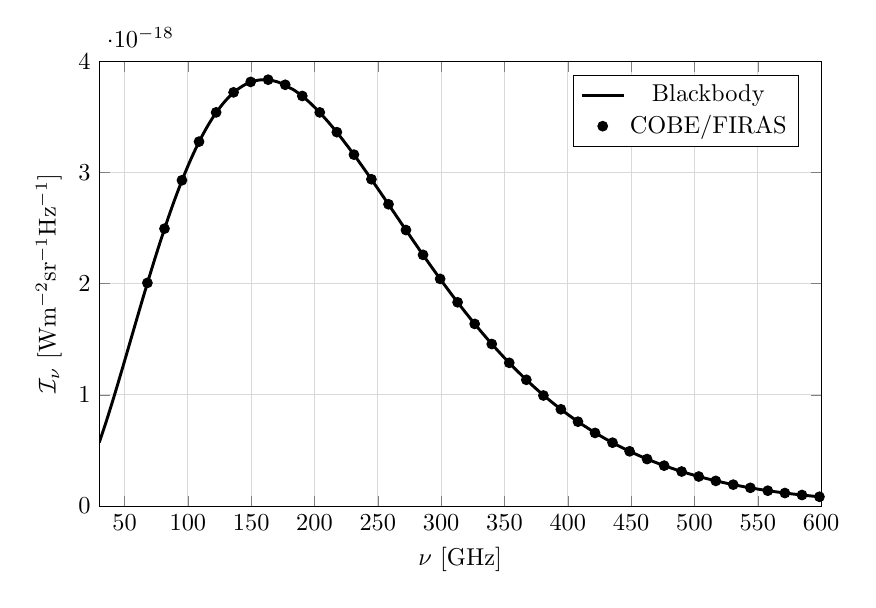
\begin{tikzpicture}[scale=.88]
  \begin{axis}[
    width=12cm, height=8cm,
    xlabel={ \(\nu\) [GHz]},
    ylabel={$\mathcal{I}_\nu$ [Wm$^{-2}$sr$^{-1}$Hz$^{-1}$]},
    xmin=30, xmax=600,
    ymin=0, ymax=4e-18,
    legend pos=north east,
    grid=both,
    major grid style={gray!30},
  ]

    % Theoretical Planck curve
    \addplot[
      domain=30:600,
      samples=300,
      very thick,
    ]
    {%
      2*6.626e-34*(x*1e9)^3/(3.00e8)^2 
      / (exp(6.626e-34*(x*1e9)/(1.381e-23*2.725)) - 1)
    };
    \addlegendentry{Blackbody}

    % Hard‑coded FIRAS‑like data with 1σ error bars
    \addplot+[
      only marks,
      mark=*,
      mark options={scale=1.0},
      black
    ]
    table[row sep=\\, x index=0, y index=1]{
      % ν [GHz]    B_ν [W/m2/sr/Hz]    σ
        68.052888 2.007230e-18\\
        81.543549 2.495080e-18\\
        95.334002 2.930240e-18\\
        108.824662 3.277700e-18\\
        122.315323 3.540810e-18\\
        136.105776 3.720790e-18\\
        149.596437 3.814930e-18\\
        163.386890 3.834780e-18\\ 
        176.877550 3.789010e-18\\
        190.368211 3.688330e-18\\
        204.158664 3.540630e-18\\
        217.649325 3.362780e-18\\
        231.139985 3.160760e-18\\
        244.930438 2.939240e-18\\
        258.421099 2.714320e-18\\ 
        272.211552 2.482390e-18\\
        285.702212 2.259400e-18\\
        299.192873 2.043270e-18\\
        312.983326 1.832620e-18\\
        326.473987 1.638300e-18\\
        339.964647 1.457500e-18\\
        353.755100 1.288350e-18\\
        367.245760 1.135680e-18\\
        380.736421 9.945100e-19\\
        394.526874 8.703600e-19\\ 
        408.017535 7.587600e-19\\
        421.508195 6.576600e-19\\
        435.298648 5.700800e-19\\
        448.789310 4.922300e-19\\
        462.579763 4.226700e-19\\
        476.070423 3.635200e-19\\
        489.860876 3.106200e-19\\
        503.351537 2.658000e-19\\
        516.842198 2.264400e-19\\
        530.632651 1.925500e-19\\
        544.123311 1.639100e-19\\
        557.913764 1.381100e-19\\
        571.404425 1.171600e-19\\
        584.895086 9.921000e-20\\
        598.685539 8.364000e-20\\
        612.176199 7.087000e-20\\
        625.666860 5.801000e-20\\ 
        639.457313 4.523000e-20\\ 
    };
    \addlegendentry{COBE/FIRAS}
  \end{axis}
\end{tikzpicture}
\caption{COBE/FIRAS \cite{COBE1996} CMB spectral radiance compared to the theoretical prediction of a blackbody radiation. COBE/FIRAS points perfectly match the curve with errors too small to be appreciated.}
\label{fig:COBE/FIRAS_spectrum}
\end{figure}

In chapter \ref{chap:SpectralDistortions} we will explore more in depth whether and how photons were in equilibrium at different times: we will discover that small distortions will be sourced in the phase space distribution, and thus also in the spectral radiance. These \textbf{spectral distortions} turn out to be smaller than the sensitivity of both COBE/FIRAS and Planck \cite{planck2018results}. 
